\documentclass{beamer}
\usepackage{ctex, hyperref}
\usepackage[T1]{fontenc}

% other packages
\usepackage{latexsym,xcolor,multicol,booktabs,calligra}
\usepackage{amsmath,amssymb,amsfonts}
\usepackage{graphicx,pstricks,listings,stackengine}
\usepackage{float}
\usepackage{subfig}
\usepackage{algorithmic}
\usepackage{algorithm}
\usepackage{multirow}

\author{学生:卢冠行~~~~指导老师:贾育衡}
\title{基于张量低秩表示的半监督子空间聚类}
\subtitle{毕业设计结题答辩}
\institute{东南大学吴健雄学院}
\date{2023年6月8日}
\usepackage{Whu}

% defs
\def\cmd#1{\texttt{\color{red}\footnotesize $\backslash$#1}}
\def\env#1{\texttt{\color{blue}\footnotesize #1}}
\definecolor{deepblue}{rgb}{0,0,0.5}
\definecolor{deepred}{rgb}{0.6,0,0}
\definecolor{deepgreen}{rgb}{0,0.5,0}
\definecolor{halfgray}{gray}{0.55}

\lstset{
    basicstyle=\ttfamily\small,
    keywordstyle=\bfseries\color{deepblue},
    emphstyle=\ttfamily\color{deepred},    % Custom highlighting style
    stringstyle=\color{deepgreen},
    numbers=left,
    numberstyle=\small\color{halfgray},
    rulesepcolor=\color{red!20!green!20!blue!20},
    frame=shadowbox,
}


\begin{document}

\kaishu
\begin{frame}
    \titlepage
    \begin{figure}[htpb]
        \begin{center}
            \includegraphics[width=0.25\linewidth]{pic/CLTlogo.jpg}
        \end{center}
    \end{figure}
\end{frame}

\begin{frame}
    \tableofcontents[sectionstyle=show,subsectionstyle=show/shaded/hide,subsubsectionstyle=show/shaded/hide]
\end{frame}


\section{课题背景}

\subsection{本文研究内容}

\begin{frame}{工作概览}

    \begin{itemize}
        \item 首次提出了一种新颖的基于张量低秩表示的半监督子空间聚类模型。
        \vspace{0.05cm}
        \item 考虑到实际应用中的不准确约束,进一步提出了鲁棒去噪聚类模型。
        \vspace{0.05cm}
        \item 所提出的模型在8个常用数据集、7个基线算法和2个评价指标上都取得了领先。
        \vspace{0.05cm}
        \item 论文已发表于\textcolor{magenta}{IEEE Transactions on Circuits and Systems for Video Technology (TCSVT)}期刊\footnote{\scriptsize\cite{10007868} Y. Jia, G. Lu, et. al, “Semi-supervised subspace clustering via tensor
low-rank representation,” IEEE TCSVT, pp. 1–1, 2023.}。
        \vspace{0.05cm}
        \item 所有主体实验代码、用到的数据集已在\href{https://github.com/GuanxingLu/Subspace-Clustering}{github}开源。
        
    \end{itemize}
\end{frame}

\subsection{子空间聚类}

\begin{frame}{子空间聚类简介}
    \vspace{-0.3cm}
    \begin{figure}[htpb]
        \centering
        \includegraphics[width=0.25\linewidth]{pic/zhiguantu4_datapart.pdf}
        \vspace{-0.4cm}
        \caption{高维数据可以被一组线性子空间的并集近似表示}
    \end{figure}

    \vspace{-0.3cm}
    \begin{itemize}
        \item 高维数据广泛存在于通信信道估计、图像处理等领域。
        \vspace{0.1cm}
        \item 这些数据通常可以用一组线性子空间的并集近似,但某个样本的子空间归属是未知的\footnote{\scriptsize\cite{5714408} R. Vidal, “Subspace Clustering,” IEEE SPM, vol. 28, no. 2, Art. no. 2, 2011.}。
        \vspace{0.1cm}
        \item 子空间聚类可以为数据样本找到对应的子空间归属,是高维数据建模的重要工具。
        
    \end{itemize}
\end{frame}

\begin{frame}{研究现状}
\begin{itemize}
    \item 基于自表示的子空间聚类是目前的研究热点。它学习自表示矩阵作为图的相似矩阵,能自适应捕捉高维数据的分布。
    \vspace{0.2cm}
    
    \item 例如,Liu等人\footnote{\cite{6180173} G. Liu, Z. Lin, S. Yan, J. Sun, Y. Yu, and Y. Ma, “Robust Recovery of Subspace Structures by Low-Rank Representation,” IEEE TPAMI, vol. 35, no. 1, Art. no. 1, 2013.}提出通过求解下述优化问题学习低秩自表示矩阵 (Low-Rank Representation, LRR)
	\begin{equation}
		\begin{aligned}
			&\min _{\mathbf{Z}, \mathbf{E} }\|\mathbf{Z}\|_{*}+\lambda\|\mathbf{E}\|_{2,1} ~\text { s.t. } \mathbf{X}=\mathbf{X Z}+\mathbf{E}.
		\end{aligned}
		\label{eq_LRR}
	\end{equation}
	
	\item 对$\mathbf{W}\!=\!(|\mathbf{Z}|\!+\!|\mathbf{Z}^{\!\top}|)\!/2$做谱聚类得到最终的聚类结果。
\end{itemize}
\end{frame}

\subsection{半监督子空间聚类}

\begin{frame}{半监督子空间聚类简介}

    \vspace{-0.3cm}
    \begin{figure}[htpb]
        \centering
        \includegraphics[width=0.25\linewidth]{pic/zhiguantu4_superpart.pdf}
        \caption{成对约束监督信息}
    \end{figure}

    \begin{itemize}
        \item 在实际应用中,一些监督信息是易获取的,如某些样本之间的成对关系。
        
        \item 这些监督信息可以表示成“必须链接”或“不能链接”的成对约束,有助于得到更有判别力的聚类结果。
 
    \end{itemize}

\end{frame}

\begin{frame}{成对约束矩阵}

    \begin{itemize}
        
        \item 可以将成对约束编码为矩阵$\mathbf{B}\in\mathbb{R}^{n\times n}$
    	\begin{equation}
    		\mathbf{B}_{ij}=\left\{\begin{aligned}
    			1, &~~\text{if}~(i, j) \in \Omega_{m} \\
    			-1, &~~\text{if}~(i, j) \in \Omega_{c}.
    		\end{aligned}\right.
    	\end{equation}
    	
        \item 对于未知的成对关系,$\mathbf{B}$的对应初始值为0。
 
    \end{itemize}

\end{frame}

\begin{frame}{研究现状}

    \begin{itemize}
        
        \item Zhuang等人\footnote{\cite{7931596} L. Zhuang, Z. Zhou, S. Gao, J. Yin, Z. Lin, and Y. Ma, “Label Information Guided Graph Construction for Semi-Supervised Learning,” IEEE TIP, vol. 26, no. 9, Art. no. 9, 2017.}直接强制具有不能链接关系样本的相似系数为0 (Semi-Supervised Low-Rank Representation, SSLRR)
        \begin{equation}
        \begin{array}{ll}
        \min _{\mathbf{Z}, \mathbf{E}} & \|\mathbf{Z}\|_{*}+\lambda\|\mathbf{E}\|_{2,1} \\
        \text { s.t. } & \mathbf{X}=\mathbf{X} \mathbf{Z}+\mathbf{E}, \\
        & \mathbf{Z}^{\top} \mathbf{1}=\mathbf{1}, \\
        & \mathbf{Z}_{i j}=0, \forall(i, j) \in \Omega_c.
        \end{array}
        \end{equation}
    	
        \item 现有工作仅从局部角度利用成对约束,即如果$\mathbf{x}_i$和$\mathbf{x}_j$有必须链接(不能链接)关系,则增大(减少)$\mathbf{Z}_{ij}$,忽略了成对约束和相似矩阵的全局结构。
 
    \end{itemize}

\end{frame}


\section{基于张量低秩表示的半监督子空间聚类方法}

\subsection{基于张量低秩表示的半监督子空间聚类模型}

\begin{frame}{所提出模型总览}

    \begin{figure}[htpb]
        \centering
        \includegraphics[width=1\linewidth]{pic/1.pdf}
        \caption{通过使用相似矩阵和成对约束矩阵相同的全局低秩结构,同时自适应地学习相似性并增强成对约束}
    \end{figure}

\end{frame}

\begin{frame}{所提出模型的数学形式}

    \begin{itemize}
            \item 所提出模型可以表述为
        
	\begin{equation}
		\begin{aligned}
			&\min _{\mathcal{C}, \mathbf{E}, \mathbf{B}, \mathbf{Z} }\|\mathcal{C}\|_{\circledast}+\lambda\|\mathbf{E}\|_{2,1}+\beta\operatorname{Tr}(\mathbf{B L B}^{\top}) \\
			&\text { s.t. } \mathbf{X}=\mathbf{X Z}+\mathbf{E}, \mathcal{C}(:,:,1)=\mathbf{Z}, \mathcal{C}(:,:,2)=\mathbf{B},  \\
			&\mathbf{B}_{i j}=s,(i, j) \in \Omega_{m}, \mathbf{B}_{i j}=-s,(i, j) \in \Omega_{c}.
		\end{aligned}
		\label{eq_origin}
	\end{equation}

            \vspace{0.2cm}
            \item 通过求解Eq. \eqref{eq_origin},联合优化相似矩阵$\mathbf{Z}$和成对约束矩阵$\mathbf{B}$,$\mathbf{B}$将把监督信息传递到$\mathbf{Z}$,同时$\mathbf{Z}$从全局角度增强$\mathbf{B}$。
    \end{itemize}
\end{frame}

\subsection{优化算法}

\begin{frame}{增广拉格朗日乘子法求解Eq. \eqref{eq_origin}}

    为了使用ADMM,引入辅助变量$\mathbf{D}$,得到Eq. \eqref{eq_origin}的等价问题
	\begin{equation}
		\begin{aligned}
			&\min_{\mathcal{C}, \mathbf{E}, \mathbf{B}, \mathbf{Z}, \mathbf{D} }\|\mathcal{C}\|_{\circledast}+\lambda\|\mathbf{E}\|_{2,1}+\beta\operatorname{Tr}(\mathbf{B L B}^{\top}) \\
			&\text { s.t. } \mathbf{X}=\mathbf{X Z}+\mathbf{E}, \mathbf{Z}=\mathcal{C}(:,:,1), \mathbf{B}=\mathcal{C}(:,:,2),\\
			&\mathbf{D}=\mathbf{B}, \mathbf{D}_{i j}=s,(i, j) \in \Omega_{m}, \mathbf{D}_{i j}=-s,(i, j) \in \Omega_{c}. 
		\end{aligned}
		\label{eq_2}
	\end{equation}

    Eq. \eqref{eq_2}的增广拉格朗日形式为
	\begin{equation}
		\begin{aligned}
			&\underset{\mathcal{C}, \mathbf{E}, \mathbf{B}, \mathbf{Z}, \mathbf{D}}{\operatorname{argmin}}\|\mathcal{C}\|_{\circledast}\!+\!\lambda\|\mathbf{E}\|_{2,1}\!+\!\beta\operatorname{Tr}(\mathbf{B L B}^{\top}) \\
			&\!+\!\frac{\mu}{2}\!(\|\mathbf{X}\!-\!\mathbf{X\!Z}\!-\!\mathbf{E}\!+\!\mathbf{Y}_{1}\!/ \mu\|_{F}^{2}\!+\!\|\mathbf{Z}\!-\!\mathcal{C}\!(:\!,\!:\!,\!1\!)\!+\!\mathcal{Y}_{2}\!(:\!,\!:\!,\!1\!)\!/\! \mu\|_{F}^{2}\\
			&+\|\mathbf{B}\!-\!\mathcal{C}(:,:,2)\!+\!\mathcal{Y}_{2}(:,:,2)\!/\! \mu\|_{F}^{2}\!+\!\|\mathbf{B}\!-\!\mathbf{D}\!+\!\mathbf{Y}_{3}\!/\!\mu\|_{F}^{2}) \\
			&\text {s.t.}~\mathbf{D}_{i j}\!=\!s,(i,j)\!\in\!\Omega_{m}, \mathbf{D}_{i j}\!=\!-\!s,(i,j)\!\in\!\Omega_{c}.
		\end{aligned}
		\label{eq_3}
	\end{equation}
\end{frame}

\begin{frame}{算法伪代码}
\begin{algorithm}[H]
        \small
		\renewcommand{\algorithmicrequire}{\textbf{输入:}}
		\renewcommand{\algorithmicensure}{\textbf{Output:}}
		\caption{利用ADMM求解Eq. \eqref{eq_origin}}
		\label{alg1}
		\begin{algorithmic}[1]
			\REQUIRE 数据 $\mathbf{X}$,成对约束 $\Omega_{m}$,$\Omega_{c}$,超参数 $\lambda$,$\beta$. 
			
			\STATE 初始化: $\mathcal{\mathcal{C}}_{0}\!=\!\mathcal{Y}_{2,0}\!=\!0$, $\mathbf{B}_{0}\!=\!\mathbf{Z}_{0}=\mathbf{D}_{0}\!=\!\mathbf{E}_{0}\!=\!\mathbf{Y}_{1,0}\!=\!\mathbf{Y}_{3,0}\!=\!0, \rho\!=\!1.1, \mu_{0}\!=\!1 \mathrm{e}\!-\!3, \mu_{\max }\!=\!1 \mathrm{e} 10$.
			
			\REPEAT
			
			\STATE 更新 $\mathcal{C}_{k+1}$;
			\STATE 更新 $\mathbf{Z}_{k+1}$;
			\STATE 更新 $\mathbf{B}_{k+1}$;
			\STATE 更新 $\mathbf{D}_{k+1}$;
			\STATE 更新 $\mathbf{E}_{k+1}$;
			\STATE 更新 $\mathbf{Y}_{1,k+1}$, $\mathcal{Y}_{2,k+1}$, $\mathbf{Y}_{3,k+1}$, 和 $\mu_{k+1}$;
			\UNTIL 收敛
		\end{algorithmic}  
	\end{algorithm}
\end{frame}


\section{实验研究}

\subsection{实验设置}

\begin{frame}
\begin{itemize}
\item 数据集:

\begin{table}[H]
    \scriptsize
	\renewcommand{\arraystretch}{1.1}
	\caption{各数据集的统计指标}
        \vspace{-0.4cm}
	\label{table_1}
	\centering
	\begin{tabular}{ccccc}
		\hline
		数据集 & 样本数 & 样本特征维度 & 类别数 & 数据类型\\
		\hline
        ORL & 400 & 1024 & 40 & 面部图像\\
        YaleB & 944 & 1024 & 15 & 面部图像\\
        COIL20 & 1440 & 1024 & 20 & 物体图像\\
        Isolet & 1560 & 617 & 26 & 语音数据\\
        MNIST & 604 & 784 & 10 & 手写字符\\
        Alphabet & 1014 & 320 & 26 & 手写字符\\
            BF0502 & 1937 & 1001 & 11 & 视频片段\\
          Notting-Hill & 1494 & 3600 & 5 & 视频片段\\
		\hline
	\end{tabular}
\end{table}

\item 基线算法:LRR与6个SoTA半监督子空间聚类算法:DPLRR, SSLRR, L-RPCA, CP-SSC, SCLRR和CLRR。

\item 评价指标:聚类准确率(Accuracy)和归一化互信息(NMI)。

\end{itemize}
\end{frame}

\subsection{实验结果}

\begin{frame}{聚类性能比较}
    \vspace{-0.2cm}
    \begin{figure}[!t]
		\subfloat[]{\includegraphics[width=2.4cm]{pic/2a.eps}
			\label{fig_1_case}}
		\subfloat[]{\includegraphics[width=2.4cm]{pic/2b.eps}
			\label{fig_2_case}}
		\subfloat[]{\includegraphics[width=2.4cm]{pic/2c.eps}
			\label{fig_3_case}}
		\subfloat[]{\includegraphics[width=2.4cm]{pic/2d.eps}
			\label{fig_4_case}}
        \quad
		\subfloat[]{\includegraphics[width=2.4cm]{pic/2e.eps}
			\label{fig_5_case}}
		\subfloat[]{\includegraphics[width=2.4cm]{pic/2f.eps}
			\label{fig_6_case}}
      \subfloat[]{\includegraphics[width=2.4cm]{pic/2g.eps}
			\label{fig_13_case}}
      \subfloat[]{\includegraphics[width=2.4cm]{pic/2h.eps}
			\label{fig_15_case}}
		\caption{不同方法在八个数据集上的聚类准确率比较}
		\label{fig_acc}
	\end{figure}

\end{frame}


\begin{frame}{相似矩阵可视化}

    \begin{figure}[!t]
		\subfloat[Proposed]{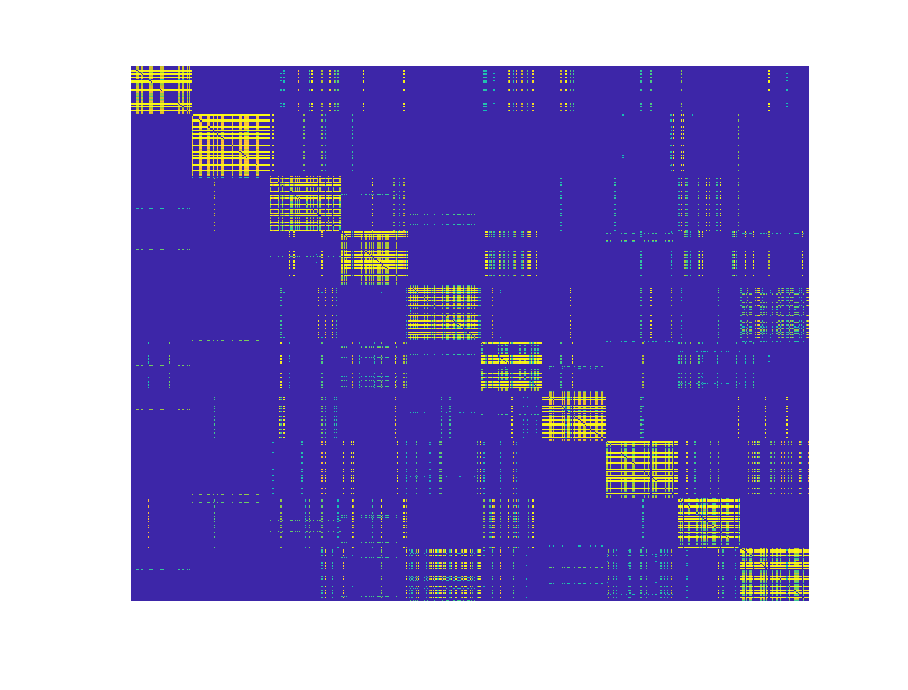
\includegraphics[width=2.2cm]{pic/4a.eps}
			\label{fig_tnn}}
		\subfloat[LRR]{\includegraphics[width=2.2cm]{pic/4b.eps}
			\label{fig_lrr}}
		\subfloat[DPLRR]{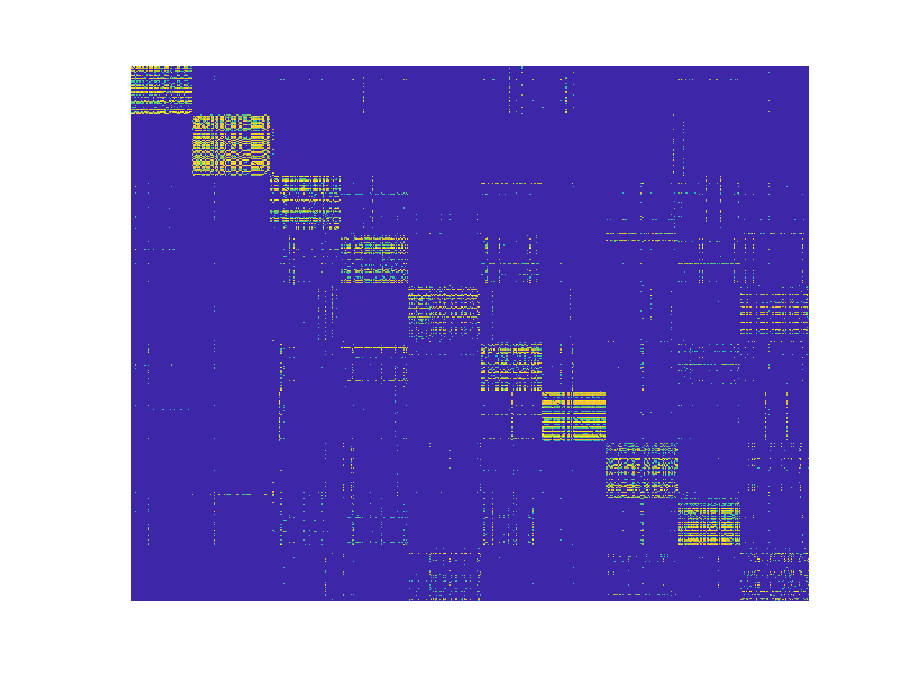
\includegraphics[width=2.2cm]{pic/4c.eps}
			\label{fig_dplrr}}
		\subfloat[SSLRR]{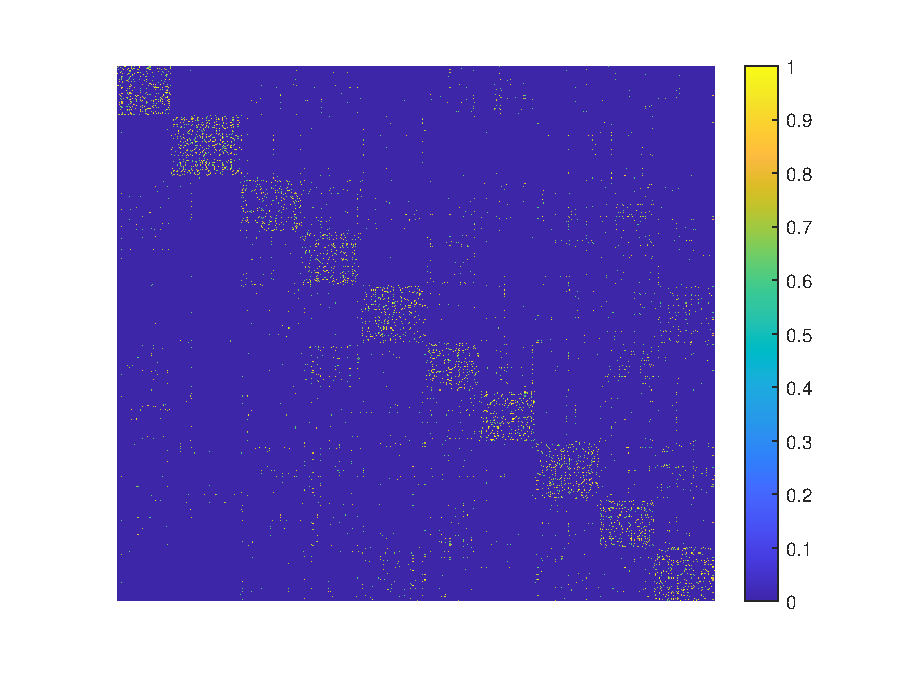
\includegraphics[width=2.2cm]{pic/4d.eps}
			\label{fig_sslrr}}
	    \quad
	    \subfloat[L-RPCA]{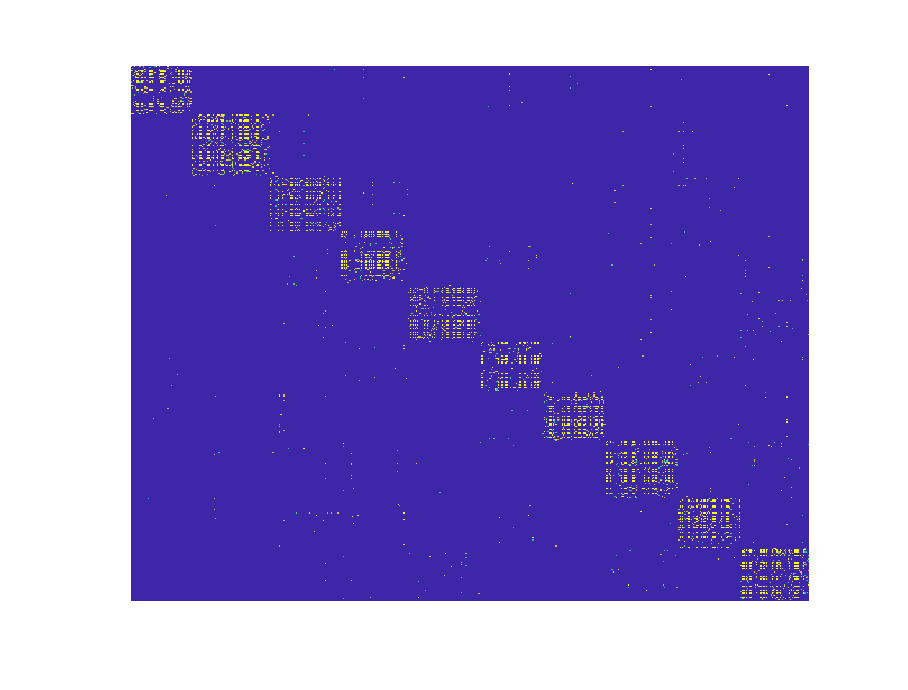
\includegraphics[width=2.2cm]{pic/4e.eps}
			\label{fig_lrpca}}
		\subfloat[CP-SSC]{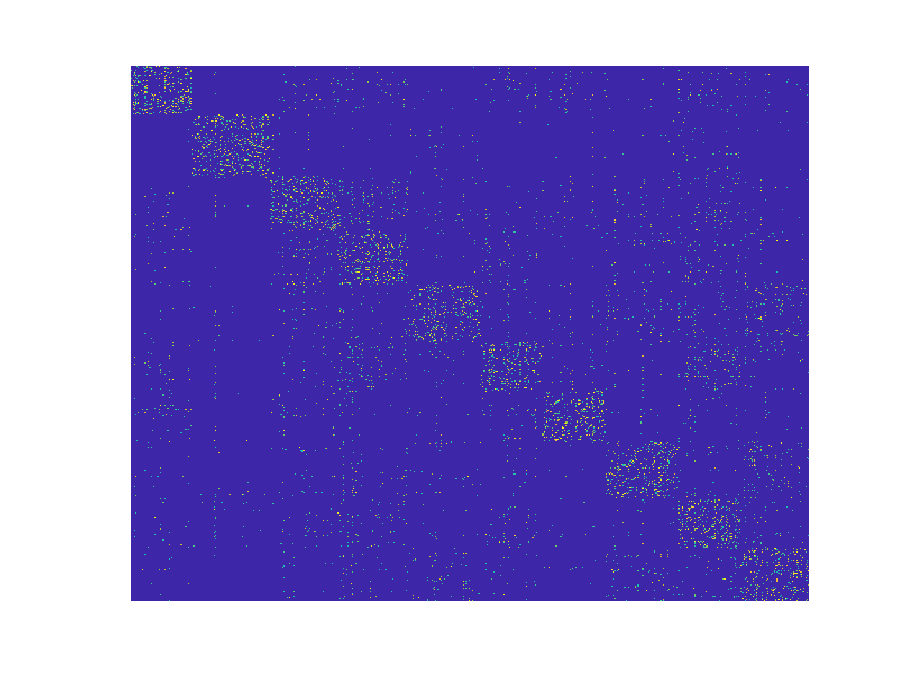
\includegraphics[width=2.2cm]{pic/4f.eps}
			\label{fig_cpssc}}
		\subfloat[SC-LRR]{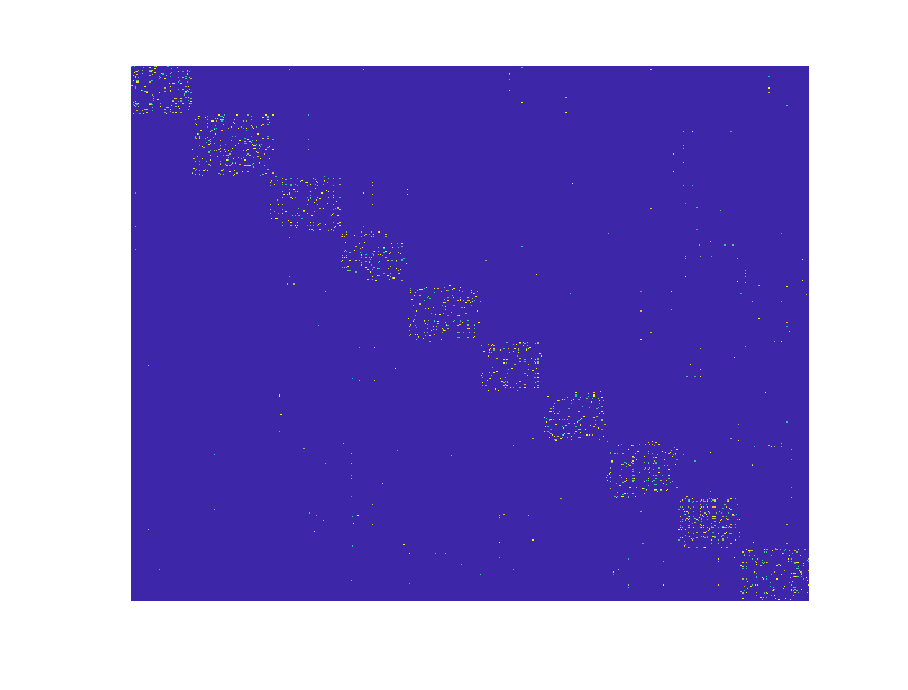
\includegraphics[width=2.2cm]{pic/4g.eps}
			\label{fig_sclrr}}
		\subfloat[CLRR]{\includegraphics[width=2.2cm]{pic/4h.eps}
			\label{fig_clrr}}
		\caption{不同方法学习的相似矩阵的可视化比较}
		\label{fig_vision}
	\end{figure}
\end{frame}


\begin{frame}{超参数分析}
    \vspace{-0.5cm}
    \begin{figure}[!t]
		\subfloat[]{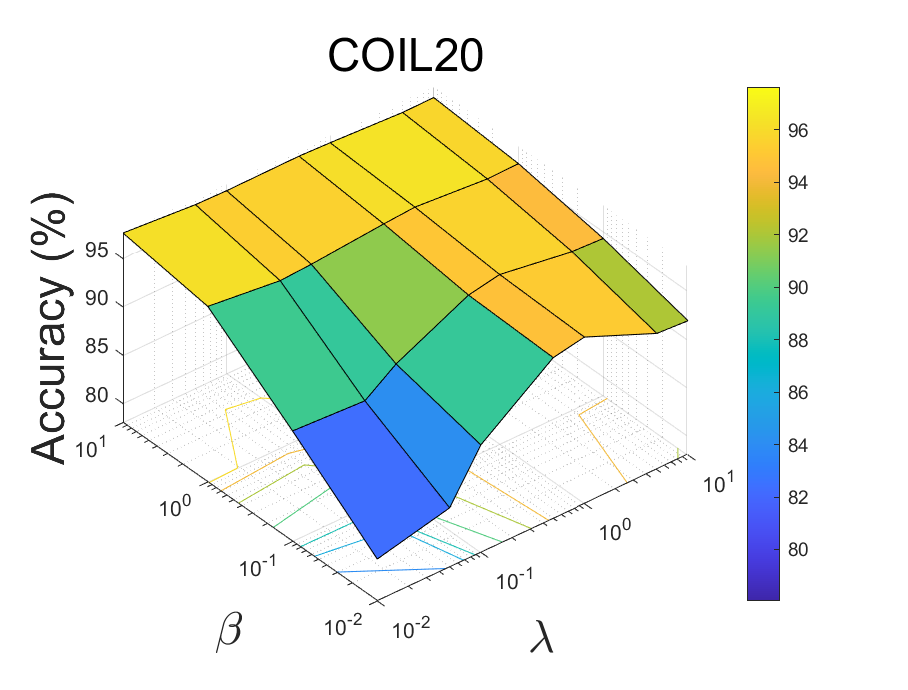
\includegraphics[width=3cm]{pic/5a.eps}}
		\subfloat[]{\includegraphics[width=3cm]{pic/5b.eps}}
		\subfloat[]{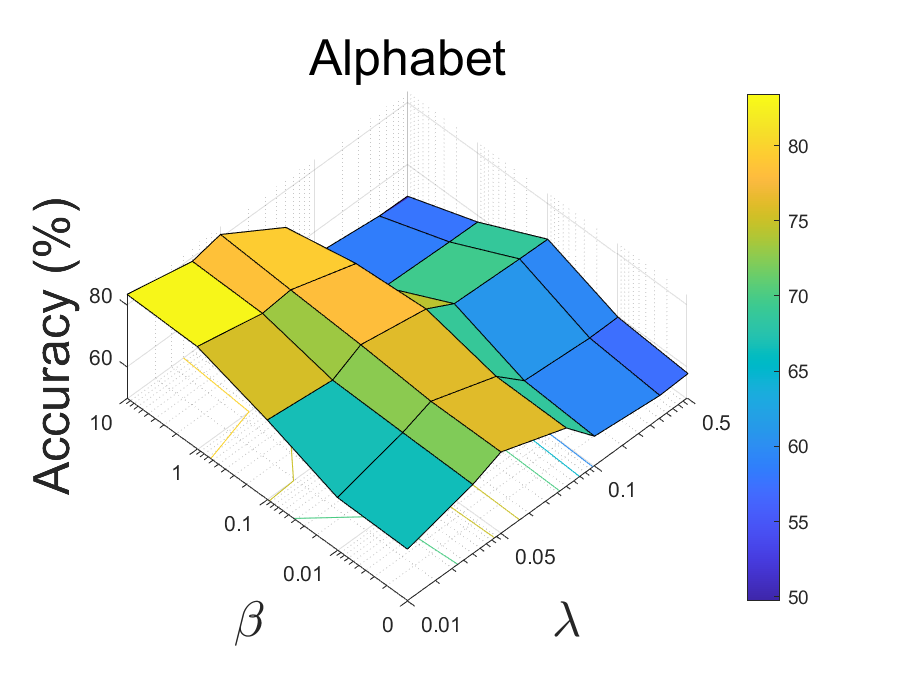
\includegraphics[width=3cm]{pic/5c.eps}}
		\caption{超参数对所提出的方法聚类准确率的影响}
		\label{fig_3}
	\end{figure}
	
	\begin{itemize}
	    \item 所提出模型对最优值附近的超参数具有较强的鲁棒性。
	    \item 建议超参数默认设置为$\lambda\!=\!0.01$和$\beta\!=\!10$。
	\end{itemize}
\end{frame}

\begin{frame}{消融实验}
\vspace{-0.25cm}
\begin{table}[H]
    \tiny
		\renewcommand{\arraystretch}{1.4}
		\setlength\tabcolsep{2pt}
		\caption{消融实验结果}
		\label{table_2}
		\centering
		\begin{tabular}{ccccccccccc}
			\hline
			百分比 & \textbf{Accuracy} & ORL & YaleB & COIL20 & Isolet & MNIST & Alphabet & BF0502 & Notting-Hill & \textbf{平均值}\\ 
			\hline
			\multirow{5}{*}{10} 
			& SSLRR & 0.7223 & 0.6965 & 0.6874 & 0.6107 & 0.5121 & 0.4278 & 0.4150 & 0.5747 & 0.5808 \\
			& CLRR & 0.7193 & 0.7032 & 0.6309 & 0.7424 & 0.5435 & 0.5120 & 0.5165 & 0.6728 & 0.6301 \\
			& 缺少图正则化 & 0.7298 & 0.7838 & 0.6744 & 0.8599 & 0.5224 & 0.5022 & 0.5786 & 0.8079 & 0.6824 \\
			& 缺少后修复处理 & 0.7298 & 0.7838 & 0.8708 & 0.8424 & 0.7659 & 0.6640 & 0.5779 & 0.9573 & 0.7740 \\
			& 完整模型 & \textbf{0.7523} & \textbf{0.8696} & \textbf{0.9171} & \textbf{0.8665} & \textbf{0.7879} & \textbf{0.6862} & \textbf{0.5915} & \textbf{0.9576} & \textbf{0.8036}\\
			
			\hline
			\multirow{5}{*}{20}
			& SSLRR & 0.7390 & 0.6998 & 0.6966 & 0.6651 & 0.5308 & 0.4672 & 0.4750 & 0.6363 & 0.6137 \\
			& CLRR & 0.7808 & 0.7130 & 0.6971 & 0.8176 & 0.6401 & 0.6064 & 0.6863 & 0.8598 & 0.7251 \\
			& 缺少图正则化 & 0.7860 & 0.9194 & 0.8101 & 0.9012 & 0.6661 & 0.6443 & 0.7554 & 0.9378 & 0.8025 \\
			& 缺少后修复处理 & 0.7860 & 0.9194 & 0.9364 & 0.9065 & 0.8366 & 0.7511 & 0.8077 & 0.9817 & 0.8657 \\
			& 完整模型 & \textbf{0.8325} & \textbf{0.9548} & \textbf{0.9569} & \textbf{0.9078} & \textbf{0.8439} & \textbf{0.7772} & \textbf{0.8223} & \textbf{0.9831} & \textbf{0.8848}
			\\
			
			\hline
			\multirow{5}{*}{30} 
			& SSLRR & 0.7600 & 0.7089 & 0.7159 & 0.7848 & 0.6538 & 0.5294 & 0.6100 & 0.7383 & 0.6876 \\
			& CLRR & 0.8160 & 0.7853 & 0.8217 & 0.8787 & 0.7030 & 0.6837 & 0.7964 & 0.9308 & 0.8020 \\
			& 缺少图正则化 & 0.8893 & 0.9664 & 0.9096 & 0.9222 & 0.8370 & 0.7671 & 0.8083 & 0.9661 & 0.8832 \\
			& 缺少后修复处理 & 0.8893 & 0.9664 & 0.9710 & 0.9300 & 0.8745 & 0.8244 & 0.8631 & 0.9917 & 0.9138 \\
			& 完整模型 & \textbf{0.8965} & \textbf{0.9742} & \textbf{0.9761} & \textbf{0.9344} & \textbf{0.8747} & \textbf{0.8355} & \textbf{0.8697} & \textbf{0.9934} & \textbf{0.9193} \\ 
			\hline
		\end{tabular}
	\end{table}

\end{frame}

\begin{frame}{收敛行为比较}

\begin{figure}[!t]
		\subfloat[]{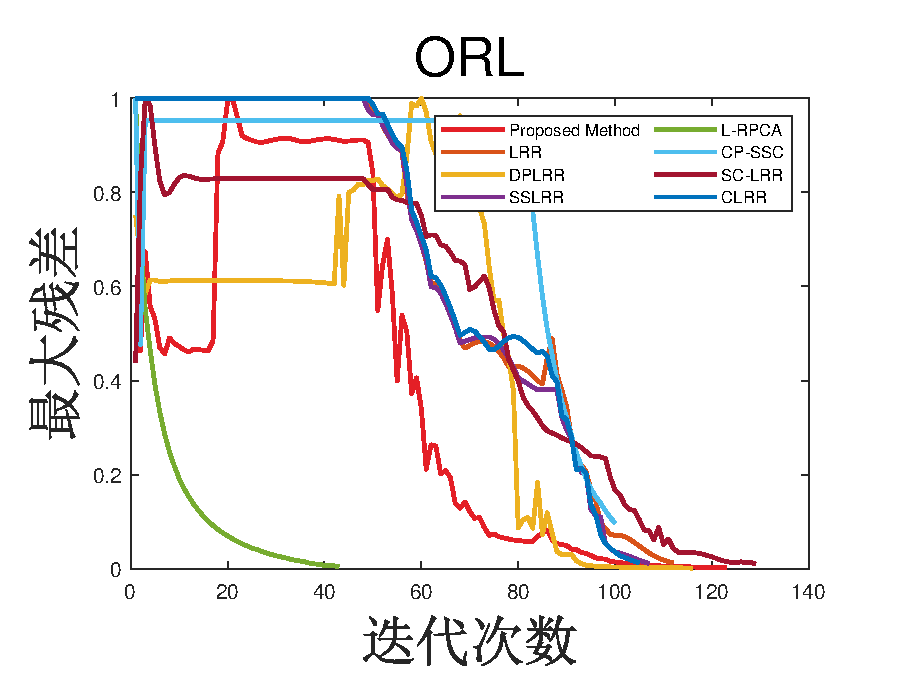
\includegraphics[width=2.4cm]{pic/6a.eps}
                \label{fig_1_converge}}
            \subfloat[]{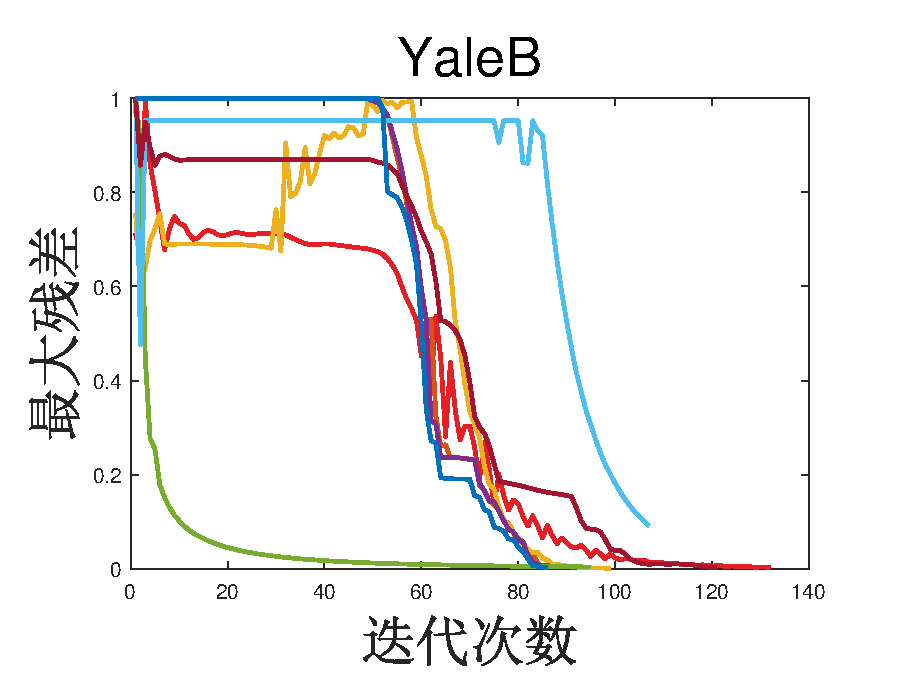
\includegraphics[width=2.4cm]{pic/6b.eps}
                \label{fig_3_converge}}
            \subfloat[]{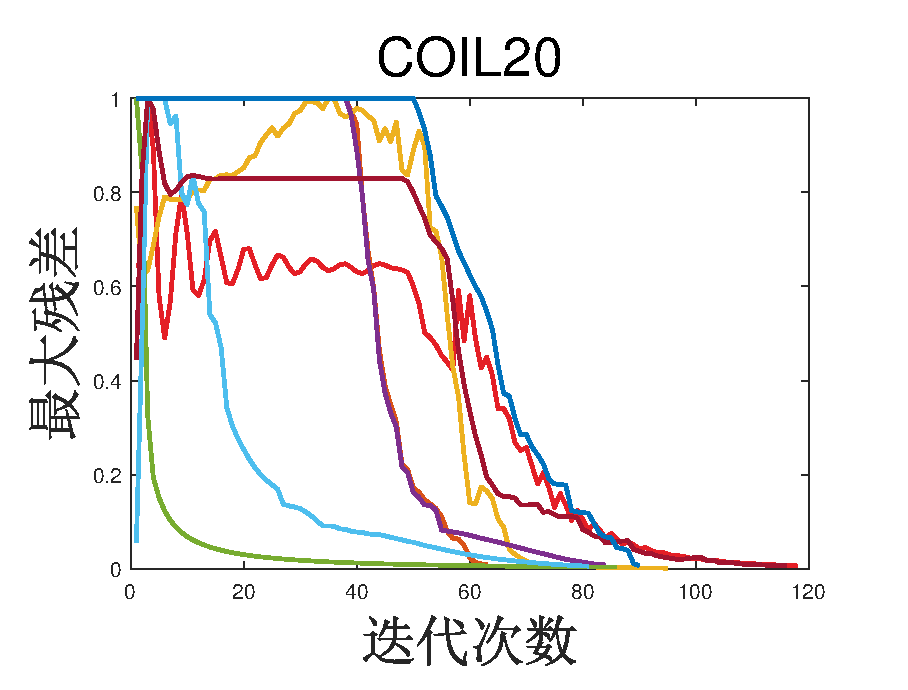
\includegraphics[width=2.4cm]{pic/6c.eps}
                \label{fig_5_converge}}
            \subfloat[]{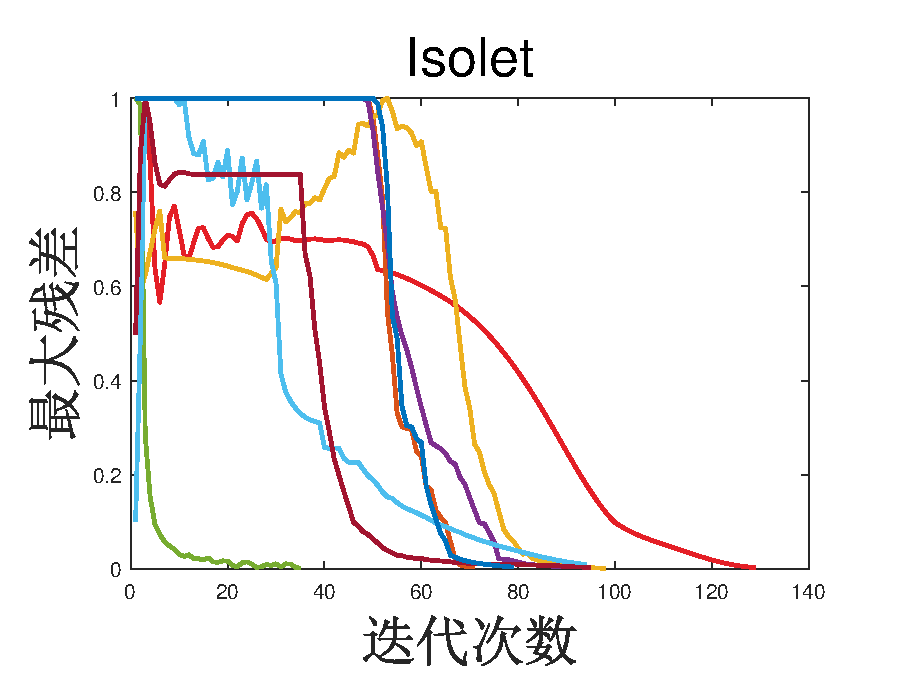
\includegraphics[width=2.4cm]{pic/6d.eps}
                \label{fig_7_converge}}
            \quad
            \subfloat[]{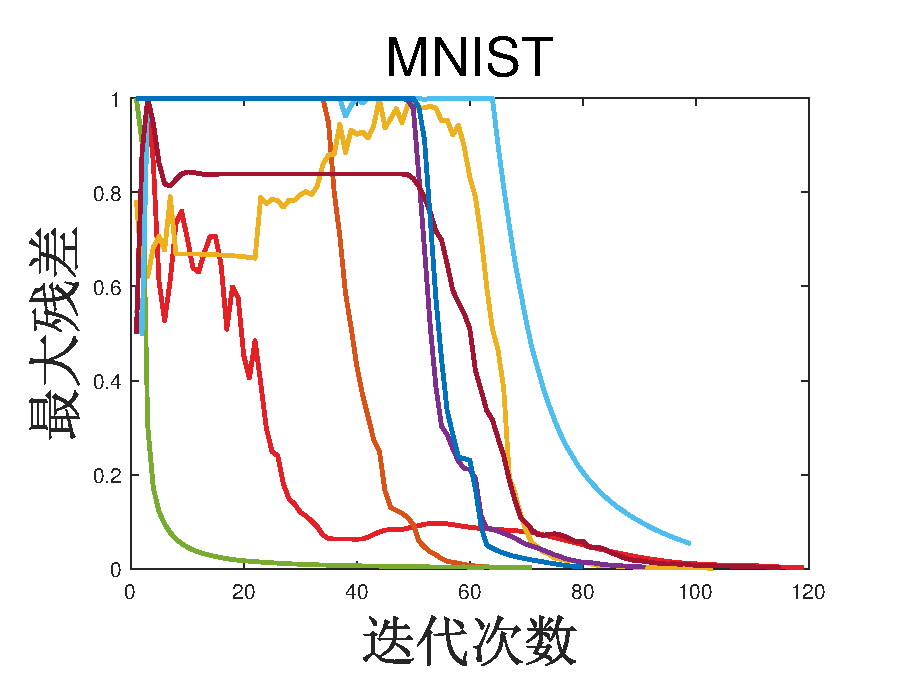
\includegraphics[width=2.4cm]{pic/6e.eps}
                \label{fig_9_converge}}
            \subfloat[]{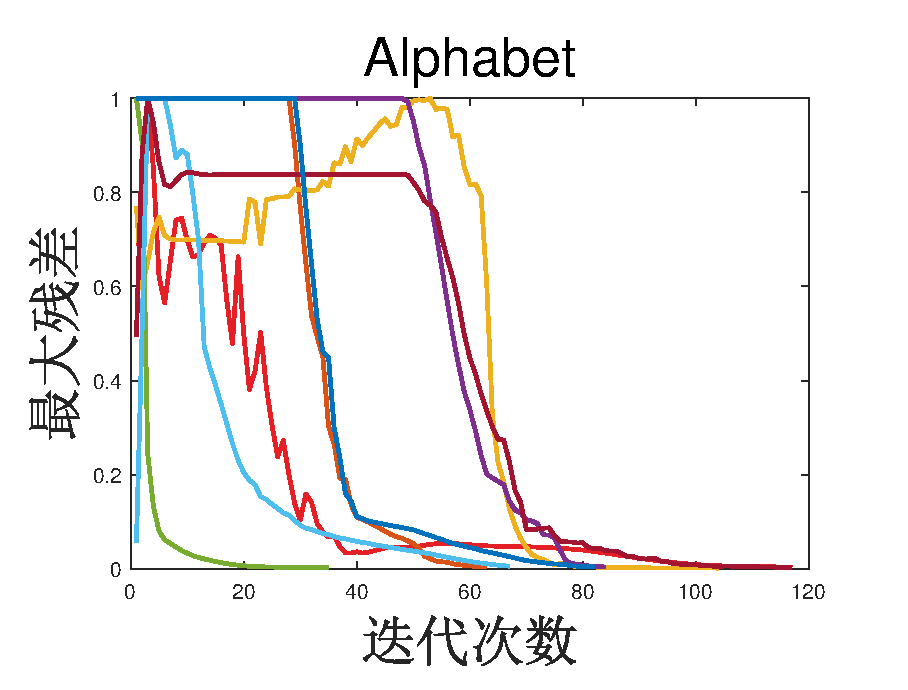
\includegraphics[width=2.4cm]{pic/6f.eps}
                \label{fig_11_converge}}
            \subfloat[]{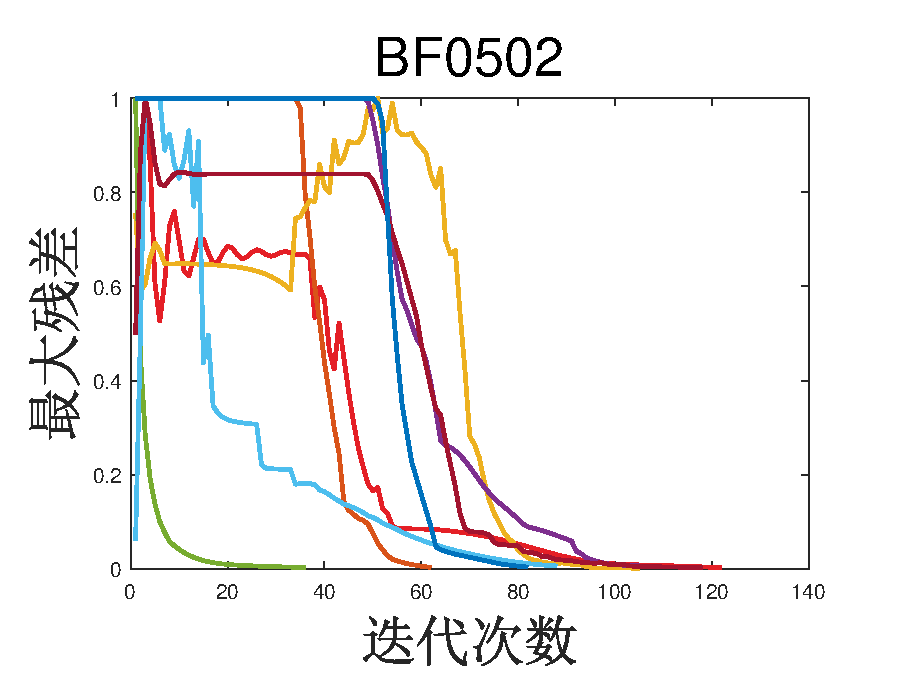
\includegraphics[width=2.4cm]{pic/6g.eps}
                \label{fig_13_converge}}
          \subfloat[]{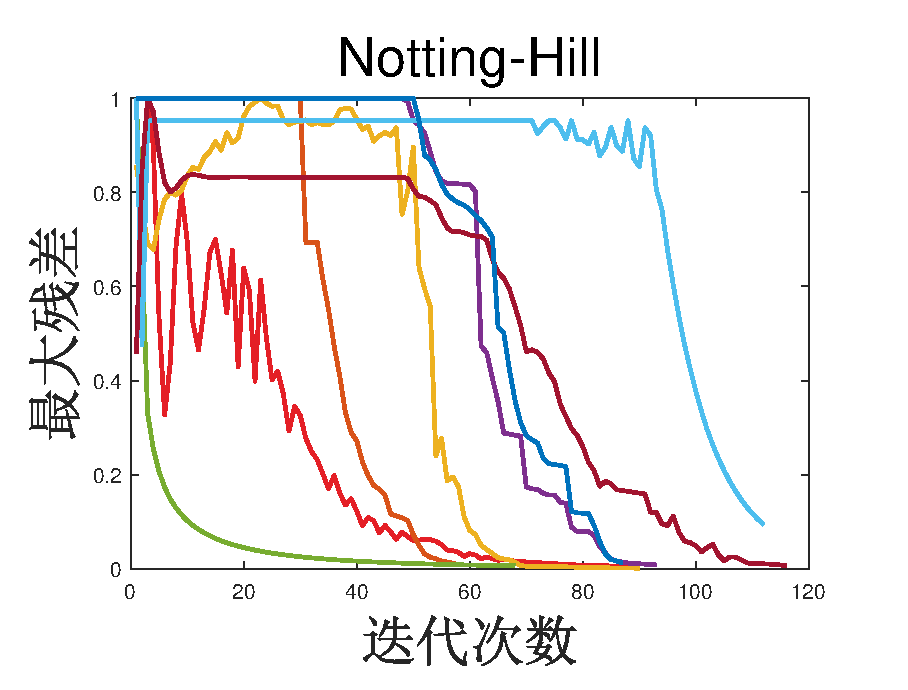
\includegraphics[width=2.4cm]{pic/6h.eps}
        \label{fig_15_converge}}
            \caption{不同方法在八个数据集上的收敛行为比较}
            \label{fig_converge}
	\end{figure}
\end{frame}

\begin{frame}{运行时间比较}

\begin{figure}[htbp]
    \centering
    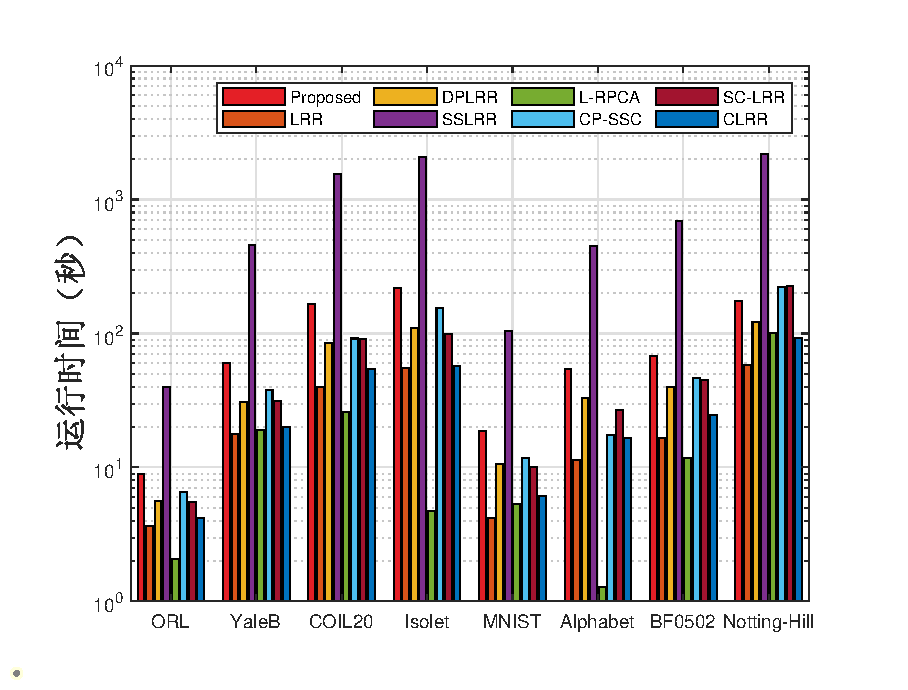
\includegraphics[width=8cm]{pic/7.eps}
    \caption{不同方法在八个数据集上的运行时间比较}
    \label{fig_time}
\end{figure}

\end{frame}

\section{参考文献}

\begin{frame}{参考文献}
    \small
    \bibliography{reference_zkj}
    \bibliographystyle{IEEEtran}  
\end{frame}

\begin{frame}
    \begin{center}
        {\Huge\calligra Thanks!}
    \end{center}
\end{frame}

\end{document}